\documentclass[a4paper,10pt]{article}
\usepackage[margin=2.5cm]{geometry}

\usepackage{amssymb,amsmath,amsthm}
\usepackage{color}
\usepackage{enumitem}
\usepackage{dsfont}
\usepackage{bm}


\newtheorem{theorem}{Theorem}
\newtheorem{proposition}{Proposition}
\newtheorem{cor}{Corollary}
\theoremstyle{definition}
\newtheorem{definition}{Definition}
\newtheorem{remark}{Remark}
\newtheorem{example}{Example}
\newtheorem{claim}{Claim}
\newtheorem{lemma}{Lemma}


%%%%%%%%%%%%%%%%%%%%%%%%%%%%%%%%%%%%%%%%%%%%%%%%%%%%%%%%%%%%%%%%%%%%%%%%%%%%%%%
% Algorithms
%%%%%%%%%%%%%%%%%%%%%%%%%%%%%%%%%%%%%%%%%%%%%%%%%%%%%%%%%%%%%%%%%%%%%%%%%%%%%%%

\usepackage{algorithm}
\usepackage{algorithmic}
\usepackage[titlenumbered,ruled,noend,algo2e]{algorithm2e}
\newcommand\mycommfont[1]{\footnotesize\ttfamily\textcolor{blue}{#1}}
\SetCommentSty{mycommfont}
\SetEndCharOfAlgoLine{}


%%%%%%%%%%%%%%%%%%%%%%%%%%%%%%%%%%%%%%%%%%%%%%%%%%%%%%%%%%%%%%%%%%%%%%%%%%%%%%%
% Code
%%%%%%%%%%%%%%%%%%%%%%%%%%%%%%%%%%%%%%%%%%%%%%%%%%%%%%%%%%%%%%%%%%%%%%%%%%%%%%%


\usepackage{fancyvrb}                  % for fancy verbatim
\usepackage{textcomp}
\usepackage[space=true]{accsupp}
% requires the latest version of package accsupp
\newcommand{\copyablespace}{
    \BeginAccSupp{method=hex,unicode,ActualText=00A0}
\ %
    \EndAccSupp{}
}
\usepackage[procnames]{listings}
% \usepackage{setspace} % need for \setstretch{1}
\lstset{%
language   = python,%
 % basicstyle = \ttfamily\setstretch{1},%
basicstyle = \ttfamily,%
columns    = flexible,%
keywordstyle=\color{javared},
firstnumber=100,
frame=shadowbox,
showstringspaces=false,
morekeywords={import,from,class,def,for,while,if,is,in,elif,
else,not,and,or,print,break,continue,return,True,False,None,access,
as,del,except,exec,finally,global,import,lambda,pass,print,raise,try,assert,!=},
keywordstyle={\color{javared}\bfseries},
commentstyle=\color{javagreen}, %vsomb_col white comments
morecomment=[s][\color{javagreen}]{"""}{"""},
upquote=true,
%% style for number
numbers=none,
resetmargins=true,
xleftmargin=10pt,
linewidth= \linewidth,
numberstyle=\tiny,
stepnumber=1,
numbersep=8pt, %
frame=shadowbox,
rulesepcolor=\color{black},
procnamekeys={def,class},
procnamestyle=\color{oneblue}\textbf,
literate={á}{{\'a}}1
{à}{{\`a }}1
{ã}{{\~a}}1
{é}{{\'e}}1
{ê}{{\^e}}1
{è}{{\`e}}1
{í}{{\'i}}1
{î}{{\^i}}1
{ó}{{\'o}}1
{õ}{{\~o}}1
{ô}{{\^o}}1
{ú}{{\'u}}1
{ü}{{\"u}}1
{ç}{{\c{c}}}1
}


\usepackage{times} % use Times

\usepackage{shortcuts_js} % possibly adapted from https://github.com/josephsalmon/OrganizationFiles/sty/shortcuts_js.sty

%%%%%%%%%%%%%%%%%%%%%%%%%%%%%%%%%%%%%%%%%%%%%%%%%%%%%%%%%%%%%%%%%%%%%%%%%%%%%%%
% IMAGES
%%%%%%%%%%%%%%%%%%%%%%%%%%%%%%%%%%%%%%%%%%%%%%%%%%%%%%%%%%%%%%%%%%%%%%%%%%%%%%%

% Use prebuiltimages/ for images extracted from code (e.g. python)
% or to share images built from a software not available by the whole team (say matlab .fig, or inskcape .svg).
% .svg files should be stored in dir srcimages/ and built from moosetex if needed:
% https://www.charles-deledalle.fr/pages/moosetex.php
% NEVER (GIT) versions files in images/ : only prebuiltimages/ & srcimages/ !

\usepackage{graphicx} % For figures
\graphicspath{{images/}, {prebuiltimages/}, {srcimages/}}
\usepackage{subcaption}


%%%%%%%%%%%%%%%%%%%%%%%%%%%%%%%%%%%%%%%%%%%%%%%%%%%%%%%%%%%%%%%%%%%%%%%%%%%%%%%
% For citations
%%%%%%%%%%%%%%%%%%%%%%%%%%%%%%%%%%%%%%%%%%%%%%%%%%%%%%%%%%%%%%%%%%%%%%%%%%%%%%%

\usepackage[authoryear]{natbib}
\usepackage{cleveref} % mandatory for no pbs with hyperlinks theorem etc...
\crefformat{equation}{Eq.~(#2#1#3)} % format for equations
\Crefformat{equation}{Equation~(#2#1#3)} % format for equations


%%%%%%%%%%%%%%%%%%%%%%%%%%%%%%%%%%%%%%%%%%%%%%%%%%%%%%%%%%%%%%%%%%%%%%%%%%%%%%%
% Header and document start
%%%%%%%%%%%%%%%%%%%%%%%%%%%%%%%%%%%%%%%%%%%%%%%%%%%%%%%%%%%%%%%%%%%%%%%%%%%%%%%


\author{Pierre-Antoine Bannier}
\title{Reweighted Multi-Task LASSO}

\begin{document}

\maketitle

\vskip 0.3in

\begin{abstract}
\textcolor{blue}{TODO}
1- we use SURE criterion to set the regulartization parameter of the reweighted Lasso
2- completely hyperparameter Free
3- extensive experiments real MEEG data
4- implementation available in MNE

\end{abstract}


%%%%%%%%%%%%%%%%%%%%%%%%%%%%%%%%%%%%%%%%%%%%%%%%%%%%%%%%%%%%%%%%%%%%%%%%%%%%%%%
% Sections in separated files
%%%%%%%%%%%%%%%%%%%%%%%%%%%%%%%%%%%%%%%%%%%%%%%%%%%%%%%%%%%%%%%%%%%%%%%%%%%%%%%

%!TEX root = ../article.tex

%%%%%%%%%%%%%%%%%%%%%%%%%%%%%%%%%%%%%%%%%%%%%%%%%%%%%%%%%%%%%%%%%%%%%%%%%%%%%%%
%%%%%%%%%%%%%%%%%%%%%%%%%%%%%%%%%%%%%%%%%%%%%%%%%%%%%%%%%%%%%%%%%%%%%%%%%%%%%%%
\section{Introduction}
\label{sec:introduction}
%%%%%%%%%%%%%%%%%%%%%%%%%%%%%%%%%%%%%%%%%%%%%%%%%%%%%%%%%%%%%%%%%%%%%%%%%%%%%%%
%%%%%%%%%%%%%%%%%%%%%%%%%%%%%%%%%%%%%%%%%%%%%%%%%%%%%%%%%%%%%%%%%%%%%%%%%%%%%%%

% Let us remind first the famous Pythagoras' theorem:

% \begin{align}\label{eq:pythagore}
% 	\norm{x+y}^2 = \norm{x}^2 + \norm{y}^2 \enspace.
% \end{align}

% Note that \Cref{eq:pythagore} is ok only under some conditions.
% In terms of visualisation, you can reference a figure easily using the command \Cref{fig:pythagore} or using Fig.~\ref{fig:pythagore}.

% \begin{figure}[h] % h stands for here
% 	\centering
% 	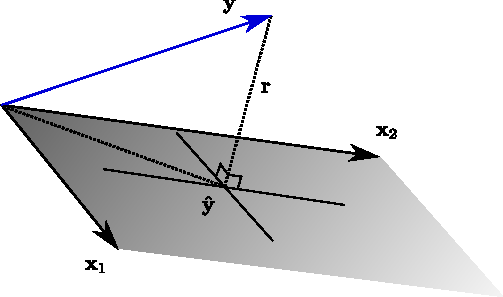
\includegraphics[width=0.6\textwidth]{residu_orth}
% 	\caption{Illustration of the residual orthogonality in least-squares.}
% 	\label{fig:pythagore}
% \end{figure}


% Also an image that is in the \texttt{prebuiltimages/} directory can also be loaded the same way:

% \begin{figure}[h] % h stands for here, ! forces even more...
% 	\centering
% 	
\includegraphics[width=0.2\textwidth]{umontpellier_logo}
% 	\caption{Illustration of a prebuiltimage available.}
% 	\label{fig:umontpellier_logo}
% \end{figure}


% For displaying side by side some images one should consider the package \lstinline+subcaptions+, that can be loaded with the \LaTeX command:

% \begin{lstlisting}[language=tex]
% \usepackage{subcaption}
% \end{lstlisting}


% \begin{figure}[t] % t stands for top (up!)
%     \centering
%     \begin{subfigure}[b]{0.33\textwidth}
%     	\centering
%         
\includegraphics[width=0.2\textwidth]{umontpellier_logo}%
%         \caption{First example}
%         \label{subfig:pythagore}
%     \end{subfigure}
%     \begin{subfigure}[b]{0.56\textwidth}
%     	\centering
%         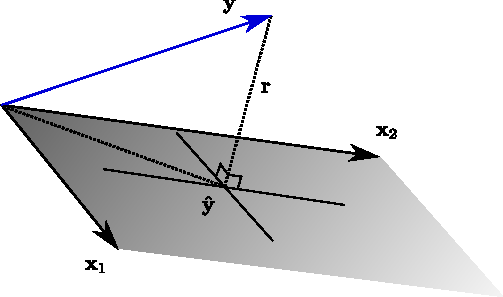
\includegraphics[width=0.5\textwidth]{residu_orth}%
%         \caption{Second example}
%         \label{subfig:logo}
%     \end{subfigure}
%     \caption{Exemples of side by side images}
%     \label{fig:double_example}
% \end{figure}

\textcolor{red}{DRAFT}

Magneto-/electroencephalography (M/EEG) allows for a non-invasive analysis of
functional brain imaging (\cite{Baillet_Mosher_Leahy_2001}). The distributed-source approach models the brain activity
with a fixed number of dipoles distributed over a dense three-dimensional 
grid within the brain volume (\cite{Dale_Sereno_1993}). The task in the inverse problem is to estimate the 
distribution of dipolar currents over this three-dimensional grid that can explain the 
measured data. Since the number of dipoles is typically much larger than the number 
of sensors placed on the skull surface of the subject, source localization is an 
ill-posed inverse problem having an infinite number of solutions. In order to render
the solution unique, biologically-plausible constraints must be applied on the optimization
problem. Literature is awash of inverse methods favoring sparse solutions to explain the
M/EEG signals including parametric (\cite{Huang_Breheny_Ma_2012}; \cite{Matsuura_Okabe_1995}; 
\cite{Uutela_Hamalainen_Somersalo_1999}) and Bayesian approaches (\cite{Costa_Batatia_Oberlin_DGiano_Tourneret_2017}; 
\cite{Oikonomou_Kompatsiaris_2020}). Those techniques are suitable for short-term source reconstruction 
- typically for tens of milliseconds after the cognitive stimulus - but fails for larger time frame when the 
stationarity assumption needs to be relaxed (\cite{Gramfort_Strohmeier_Haueisen_Hamalainen_Kowalski13}). 
In recent years, a promising approach has been Mixed Norm Estimate (MxNE) 
(\cite{Gramfort_Kowalski_Hamalainen12}), that extends the Lasso (\cite{Tibshirani96}), 
a regularized least-square model that applies a $\ell_1$-norm penalty on the coefficients to yield 
sparse solutions. More precisely, MxNE is a multi-task Lasso
model that imposes a block separable convex penalty with a $\ell_{2,1}$-mixed-norm, similar to 
Group Lasso (\cite{Yuan_Lin06}) or Group Basis Pursuit (\cite{Liao_Li_Carin_2014}). We refer to 
\cite{Bach_Jenatton_Mairal_Obozinski12} for a comprehensive review of sparsity-inducing norms. 
Each block represents the source activation over time of a dipole with fixed or free orientation at a specific source location.
\cite{Strohmeier_Bekhti_Haueisen_Gramfort_2016} improved MxNE by proposing iteratively reweighted Mixed Norm Estimate 
(irMxNE), a M/EEG sparse source imaging approach based on the iterative reweighting of the $\ell_1$-
norm (\cite{Candes_Wakin_Boyd08}), that showed state-of-the-art results on the source localization
problem.

All those approaches are parametrized by one hyperparameter that controls the sparsity level
induced by the constraint. Figure 1 shows the critical effect of this regularizing hyperparameter 
on the sparsity of the solution. The larger the hyperparameter, the sparser the solution which translates
into fewer sources recovered by the model. Hyperparameter selection remains a challenging yet crucial task
for inverse problems. Various approaches have been proposed to automatically select the regularizing 
hyperparameter in sparse models. Bayesian approaches consist in setting a prior distribution 
and select the hyperparameter by \textit{maximum-a-posteriori} (MAP) estimation (\cite{Pereyra_BioucasDias_Figueiredo_2015};
\cite{Vidal_Bortoli_Pereyra_Durmus_2020}).
\cite{Pereyra_BioucasDias_Figueiredo_2015} introduced two hierarchical Bayesian methods to perform MAP 
inference when the value of the regularization parameter is unknown, by setting a Gamma prior on the 
unknown hyperparameter. \cite{Bekhti_Badeau_Gramfort_2017} adapted this method to the multi-task Lasso problem
for source localization and proposed a method to adjust the scale parameters $\alpha$ and $\beta$
of the Gamma prior. However, both methods require to fine-tune at least one parameter by hand, which is a
tedious process for non-experts. Hyperparameter selection can also be done using an exhausive
grid-search using a held-out criterion (\cite{Bergstra_Bengio12}, \cite{BergstraBardenetBengioKegl2011}), 
the chosen hyperparameter is the one that minimizes this criterion. \cite{Pedregosa16} has 
showed that cross-validating the hyperparameter on held-out sets is not a suitable approach for inverse 
problems. Figure 2 shows that cross-validation (CV) consistently performs worse than other 
hyperparameter selection methods. CV requires the i.i.d. assumption to be fulfilled, which is 
not the case when dealing with an array of spatially-correlated sensors. The crucial question revolves around
finding a good estimator of the reconstruction error of a model. \cite{Stein81} proposed an unbiased estimator
of the quadratic risk of models, called the Stein's Unbiased Risk Estimator (SURE). The SURE has proved to be 
useful for digital signal and image reconstruction (\cite{Pesquet_Benazza_Chaux_2009}) and for
parameter selection (\cite{Deledalle_Vaiter_Fadili_Peyre14}). In this paper, we propose a procedure based 
on the Monte-Carlo finite difference SURE (\cite{Deledalle_Vaiter_Fadili_Peyre14}) that achieves 
state-of-the-art performance on hyperparameter selection tasks for MxNE and irMxNE,
both on simulated and real M/EEG data. Then we adapt this procedure to the time-frequency domain
with TF-irMxNE. An implementation of our code can be found in MNE software (\cite{mne}).
The different strategies are tested on simulations and multiple source reconstruction 
problems using public M/EEG data.
%
\newline
\newline
%
\textit{\textbf{Notation}} The transpose of a matrix $\mathbf{A} \in \mathbb{R}^{M \times N}$ is
denoted $\bf{A}^\top$. $\mathbf{A}[i,:]$ and $\mathbf{A}[:,j]$ correspond to the $i^{th}$
row and the $j^{th}$ column respectively. $\norm{A}_{\text{F}}$ indicates the Frobenius norm,
and $\norm{\mathbf{A}}_{p,q}$ the $\ell_{p,q}$-mixed-norm with $\norm{\mathbf{A}}_{p,q} 
= \left(\sum_i \left(\sum_j \lvert \mathbf{A}[i,j] \rvert^p\right)^{q/p}\right)^{1/q}$.
$\mathbf{I}$ denotes the identity matrix.


%%%%%%%%%%%%%%%%%%%%%%%%%%%%%%%%%%%%%%%%%%%%%%%%%%%%%%%%%%%%%%%%%%%%%%%%%%%%%%%
\subsection{Background}
\label{sub:background}
%%%%%%%%%%%%%%%%%%%%%%%%%%%%%%%%%%%%%%%%%%%%%%%%%%%%%%%%%%%%%%%%%%%%%%%%%%%%%%%
%

\subsubsection{The multi-task Lasso regression model}

The M/EEG source localization problem can be written as:

\begin{equation}
    \mathbf{M = GX + E}
\end{equation}
%
where $\mathbf{M} \in \mathbb{R}^{N \times T}$ is a measurement matrix where $N$ is the
number of sensors placed on the skull surface and $T$ is the number of time instants.
$\mathbf{G} \in \mathbb{R}^{N \times S}$ is the design matrix, a known 
instantaneous mixing matrix also called the gain matrix. This matrix relates the source
to the measurements. $\mathbf{E} \in \mathbb{R}^{N \times T}$ is the noise matrix, which
is assumed to be additive, white and Gaussian, $\mathbf{E}[:,j] \sim \mathcal{N}(0, \mathbf{I})
\enspace \forall j$. $\mathbf{X} \in \mathbf{R}^{S \times T}$ is the coefficient matrix to be estimated. 
It corresponds at every point in time to the estimated current intensity at the dipoles in
the brain volumes.
\\
Assuming a known regularization parameter $\lambda > 0$, we recall the multi-task
Lasso regression model defined by:

\begin{equation}
    \mathbf{X}_{\lambda}^* \in \argmin_{\mathbf{X}}
    \frac{1}{2}\norm{\mathbf{M - GX}}^2_{\text{F}}
    + \lambda \mathcal{P}(\mathbf{X})
    \enspace ,
\end{equation}
%
where $\mathcal{P}(\mathbf{X})$ is a regularization term and $\lambda$ the hyperparameter
that controls the trade-off between the data-fit and the penalization. In practice, the solution
$\hat{\mathbf{X}}_{\lambda}$ relies heavily on $\lambda$ (see Figure 1).

\subsubsection{The bi-level optimization framework}

The hyperparameter selection problem can be cast into a bi-level optimization framework. We refer 
to \cite{Pedregosa16} for a comprehensive review of bi-level hyperparameter optimization problems.
We denote $\mathcal{L}$ the criterion we wish to optimize w.r.t. $\lambda$ (e.g. a SURE-based criterion) 
referred as the outer loss, and $L$ a cost function of the coefficient matrix $\mathbf{X}$ referred
as the inner loss. Therefore, we can write the hyperparameter optimization problem as the 
nested bi-level optimization problem:

\begin{align*}
    &\lambda^* \in \argmin_{\lambda} 
    \Biggl\{
        \mathcal{L}(\lambda) 
        \triangleq 
        \mathcal{C}(\mathbf{X}_{\lambda}^*)
    \Biggr\} \\
    &\text{s.t.} \quad 
    \mathbf{X}_{\lambda}^* 
    \in 
    \argmin_{\mathbf{X}} L(\mathbf{X}, \lambda)
    \enspace .
\end{align*}
%


\subsubsection{SURE, a surrogate of the quadratic risk}

\begin{itemize}
    \item Optimization problems (non-convex)
    \item Problem bilevel de la crossval
    \item Dire en detail pq la crossval "c'est pas bien", donner un exemple
    \item SURE: expliquer pourquoi le SURE et les différentes techniques d'approx du SURE
\end{itemize}
%
%
%
%
%%%%%%%%%%%%%%%%%%%%%%%%%%%%%%%%%%%%%%%%%%%%%%%%%%%%%%%%%%%%%%%%%%%%%%%%%%%%%%%
\subsection{Experience}
\label{sub:experience}
%%%%%%%%%%%%%%%%%%%%%%%%%%%%%%%%%%%%%%%%%%%%%%%%%%%%%%%%%%%%%%%%%%%%%%%%%%%%%%%
%

%%%%%%%%%%%%%%%%%%%%%%%%%%%%%%%%%%%%%%%%%%%%%%%%%%%%%%%%%%%%%%%%%%%%%%%%%%%%%%%
\subsection{Implementation details}
\label{sub:experience}
%%%%%%%%%%%%%%%%%%%%%%%%%%%%%%%%%%%%%%%%%%%%%%%%%%%%%%%%%%%%%%%%%%%%%%%%%%%%%%%
%
Free fixed solver
Warm start

\clearpage

% ...more text here.
%!TEX root = ../article.tex


%%%%%%%%%%%%%%%%%%%%%%%%%%%%%%%%%%%%%%%%%%%%%%%%%%%%%%%%%%%%%%%%%%%%%%%%%%%%%%%
%%%%%%%%%%%%%%%%%%%%%%%%%%%%%%%%%%%%%%%%%%%%%%%%%%%%%%%%%%%%%%%%%%%%%%%%%%%%%%%
\section{Algorithms}
\label{sec:algorithms}
%%%%%%%%%%%%%%%%%%%%%%%%%%%%%%%%%%%%%%%%%%%%%%%%%%%%%%%%%%%%%%%%%%%%%%%%%%%%%%%
%%%%%%%%%%%%%%%%%%%%%%%%%%%%%%%%%%%%%%%%%%%%%%%%%%%%%%%%%%%%%%%%%%%%%%%%%%%%%%%

% Considering the techniques mentioned by \citet{Jaggi13}, you can use a different algorithm a in say \Cref{alg:DC}



% {\fontsize{4}{4}\selectfont
% \begin{algorithm}[h]  % again h stands for here
% \SetKwInOut{Input}{input}
% \SetKwInOut{Init}{init}
% \SetKwInOut{Parameter}{param}
% \caption{\textsc{Implicit differentiation}
% }
% %
% \Input{$
%     X \in \bbR^{n \times p},
%     y \in \bbR^{n},
%     \lambda \in \bbR,
%     n_{\text{iter}} \in \bbN$}
%     \tcp{jointly compute coef. and Jacobian}

%     \If{Lasso}{
%     Get $\beta = Lasso(X, y, \lambda, n_{\text{iter}})
%     $ and its support $\hat S$.

%     $\hat J_{\phantom{\hat S}} = 0_{p}$
%     \tcp{affectation}

%     $\hat J_{\hat S} =
%     - n e^\lambda (X_{\hat S}^\top X_{\hat S})^{-1} \sign \beta_{\hat S} $
%     }
%     \If{wLasso}{
%     Get $\beta = wLasso(X, y, \lambda, n_{\text{iter}})
%     $ and its support $\hat S$.

%     $\hat J = 0_{p \times p}$

%     $\hat J_{\hat S, \hat S} =
%     - (X_{\hat S}^\top X_{\hat S})^{-1}
%     \diag ( n e^{\lambda_{\hat S}}
%     \odot \sign \beta_{\hat S})$
%     }
% \For{$k = 0,\dots, n_{\text{iter\_jac}} - 1$
%     }{a = 1}

% \Return{$\beta, \hat J$}
% \label{alg:compute_jac_implicit_diff}
% \end{algorithm}
% }


% It is also possible to use the standard citation style \cite{Tibshirani96}.


%!TEX root = ../article.tex

%%%%%%%%%%%%%%%%%%%%%%%%%%%%%%%%%%%%%%%%%%%%%%%%%%%%%%%%%%%%%%%%%%%%%%%%%%%%%%%
%%%%%%%%%%%%%%%%%%%%%%%%%%%%%%%%%%%%%%%%%%%%%%%%%%%%%%%%%%%%%%%%%%%%%%%%%%%%%%%
\section{Experiments}
\label{sec:experiments}
%%%%%%%%%%%%%%%%%%%%%%%%%%%%%%%%%%%%%%%%%%%%%%%%%%%%%%%%%%%%%%%%%%%%%%%%%%%%%%%
%%%%%%%%%%%%%%%%%%%%%%%%%%%%%%%%%%%%%%%%%%%%%%%%%%%%%%%%%%%%%%%%%%%%%%%%%%%%%%%


% Also an image that is in the \texttt{prebuiltimages/} directory can also be loaded the same way:

% \begin{figure}[h] % h stands for here, ! forces even more...
% 	\centering
% 	
\includegraphics[width=0.2\textwidth]{umontpellier_logo}
% 	\caption{Illustration of a prebuiltimage available.}
% 	\label{fig:umontpellier_logo}
% \end{figure}


% For displaying side by side some images one should consider the package \lstinline+subcaptions+, that can be loaded with the \LaTeX command:

% \begin{lstlisting}[language=tex]
% \usepackage{subcaption}
% \end{lstlisting}


% \begin{figure}[t] % t stands for top (up!)
%     \centering
%     \begin{subfigure}[b]{0.33\textwidth}
%     	\centering
%         
\includegraphics[width=0.2\textwidth]{umontpellier_logo}%
%         \caption{First example}
%         \label{subfig:pythagore}
%     \end{subfigure}
%     \begin{subfigure}[b]{0.56\textwidth}
%     	\centering
%         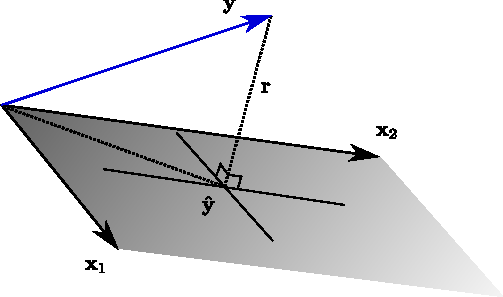
\includegraphics[width=0.5\textwidth]{residu_orth}%
%         \caption{Second example}
%         \label{subfig:logo}
%     \end{subfigure}
%     \caption{Exemples of side by side images}
%     \label{fig:double_example}
% \end{figure}

\subsection{MSE, SURE and F1 score baseline}

\begin{figure}[h]
    \centering
    
\includegraphics[scale=0.5]{metric_comparison/sure_mse_f1_comparison_legend}
    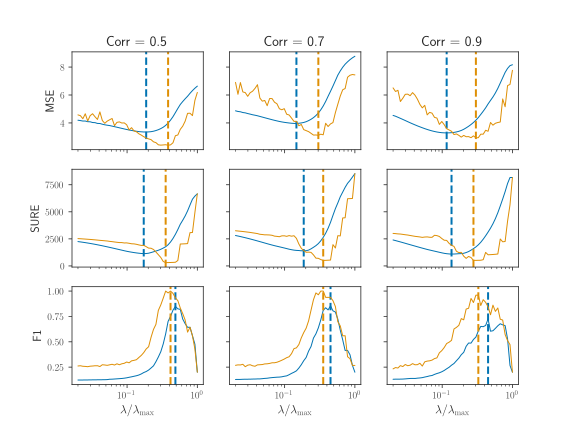
\includegraphics[scale=0.5]{metric_comparison/sure_mse_f1_comparison}
    \caption{SURE, MSE, F1 comparison, \textcolor{blue}{TODO explain more in legend}}
    \label{fig:sure_mse_f1_comparison}
\end{figure}

\subsection{Left-Auditory experiments}


\begin{figure}
    \centering
    %
    \begin{subfigure}[t]{0.4\textwidth}
        \centering
        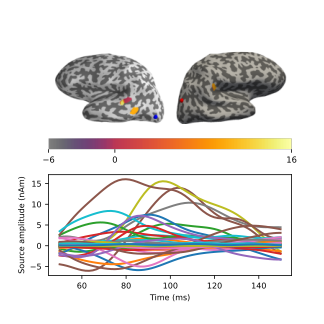
\includegraphics[scale=0.6]{blobs/blob-left_auditory-lasso-cv}
        \caption{Held-out MSE loss}
        \label{subfig:left_auditory_lasso_cv}
    \end{subfigure}
    %
    \hfill
    %
    \begin{subfigure}[t]{0.4\textwidth}
        \centering
        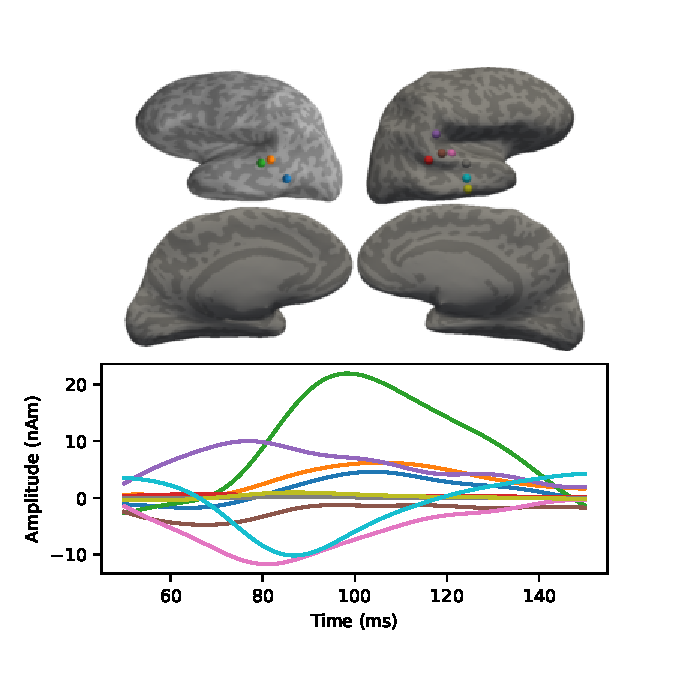
\includegraphics[scale=0.6]{blobs/blob-left_auditory-lasso-sure}
        \caption{SURE}
        \label{subfig:left_auditory_lasso_sure}
    \end{subfigure}

    \caption{Multi-Task LASSO}
\end{figure}

\begin{figure}
    \centering
    %
    \begin{subfigure}[t]{0.4\textwidth}
        \centering
        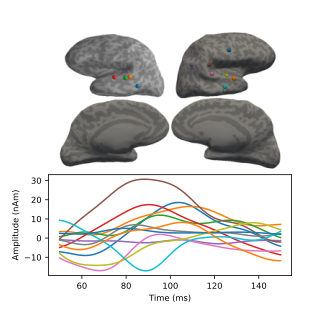
\includegraphics[scale=0.6]{blobs/blob-left_auditory-adaptive-cv}
        \caption{Held-out MSE loss}
        \label{subfig:left_auditory_adaptive_cv}
    \end{subfigure}
    %
    \hfill
    %
    \begin{subfigure}[t]{0.4\textwidth}
        \centering
        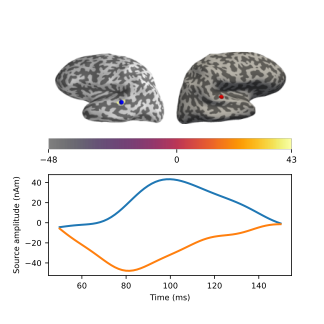
\includegraphics[scale=0.6]{blobs/blob-left_auditory-adaptive-sure}
        \caption{SURE}
        \label{subfig:left_auditory_adaptive_sure}
    \end{subfigure}

    \caption{Reweighted Multi-Task LASSO}
\end{figure}



% if needed add appendix here:
% \input{content/appendix}

\newpage
\bibliographystyle{plainnat}
\bibliography{../biblio/references_all}
% see https://github.com/josephsalmon/OrganizationFiles/biblio/references_all.bib, or adapt your own from that one.

\end{document}
